\section{Исследовательский раздел}
В исследовательском разделе будут проведены замеры времени для разных конфигураций камеры и зеркального кубика рубика. В дальнейшем, такая конфигурация будет называться кадром.

\subsection{Характеристики ПК}
Все дальнейшие замеры времени будут проведены на настольном персональном компьютере, имеющем характеристики:
\begin{itemize}
	\item процессор --- AMD Ryzen 7 1700X, 3.4 ГГц \cite{bib:processor};
	\item ОЗУ --- 16ГБ DDR4-2133, 1066 МГц;
	\item видеокарта --- AMD Radeon RX 570, 8 Гб GDDR5, ядро 1250 МГц, память 1750 МГц \cite{bib:graphics-card}.
\end{itemize}

\subsection{Результаты измерения времени}
В таблице \ref{tbl:time_measures} представлены результаты замеров времени, проведённых для кадров, представленных на рисунках \ref{fig:test1}, \ref{fig:test2}, \ref{fig:test3}, \ref{fig:test4}, \ref{fig:test5} и \ref{fig:test6} соответственно.

\begin{table}[!ht]
 	\centering
 	\caption{Результаты замеров времени}
 	\label{tbl:time_measures}
 	\begin{tabular}{|c|c|c|}
 		\hline
 		№ кадра & Число пикселей & Время в миллисекундах \\
 		\hline
 		1 & 1578260 & 52718.7 \\
 		2 & 1578260 & 42159.7 \\
 		3 & 1578260 & 36643.9 \\
 		4 & 1578260 & 56138.4 \\
 		5 & 1578260 & 48544.3 \\
 		6 & 1578260 & 48345.9 \\
 		\hline
 	\end{tabular}
 \end{table}

\begin{figure}
	\centering
	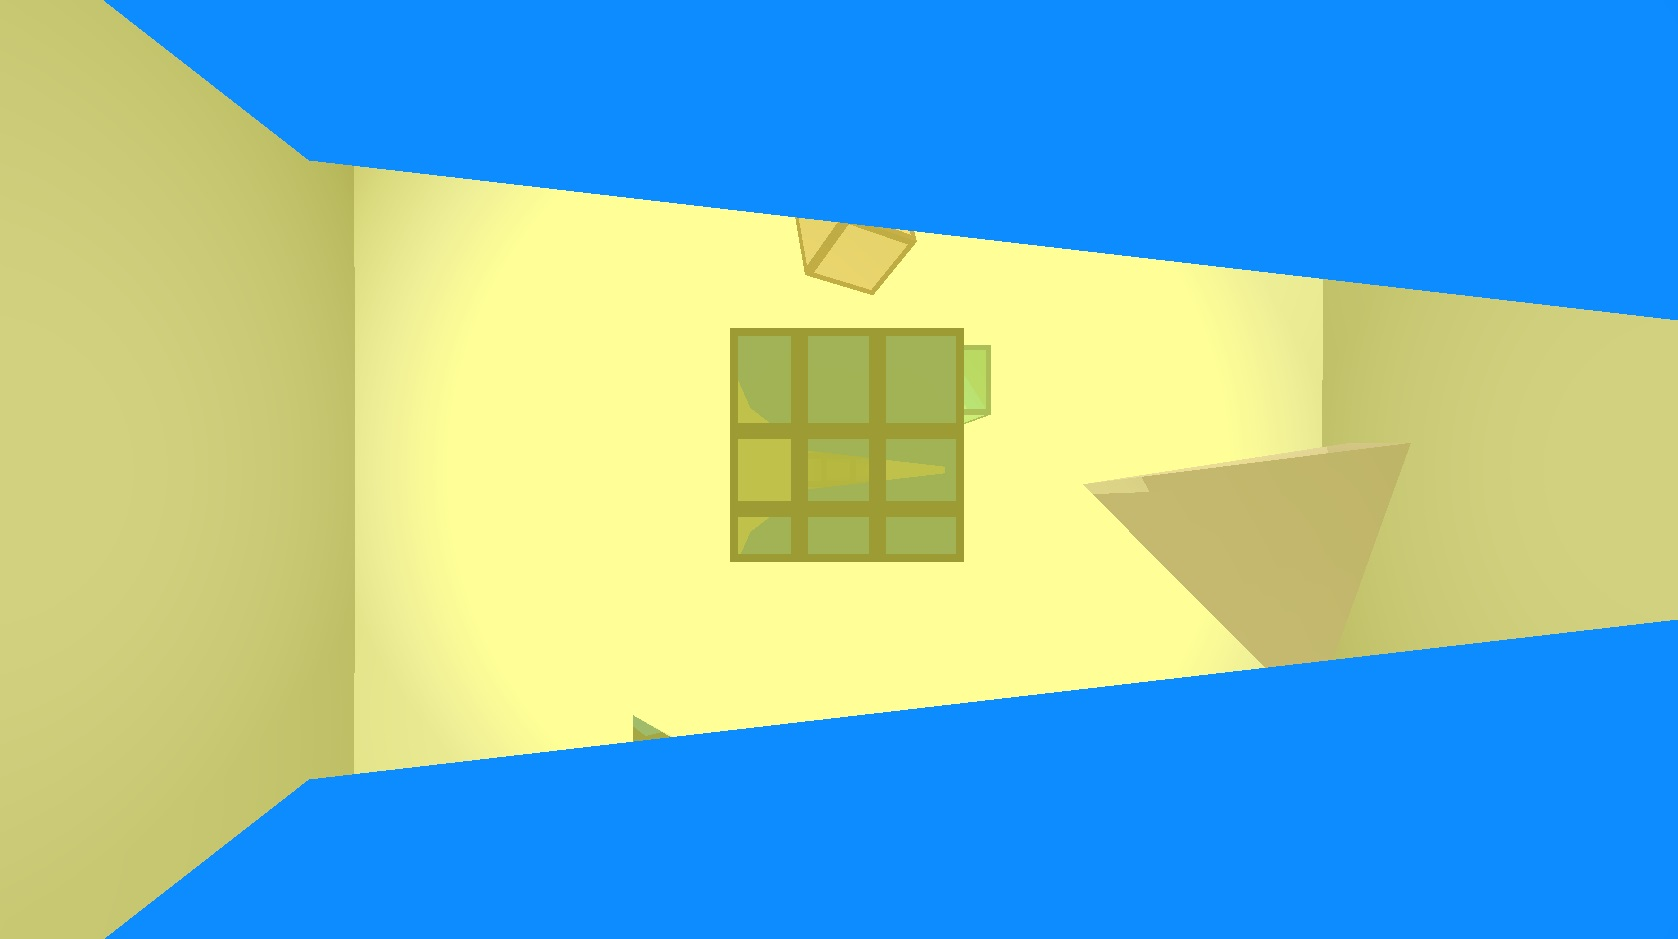
\includegraphics[width=1\linewidth]{test1}
	\caption{Кадр для теста №1}
	\label{fig:test1}
\end{figure}

\begin{figure}
	\centering
	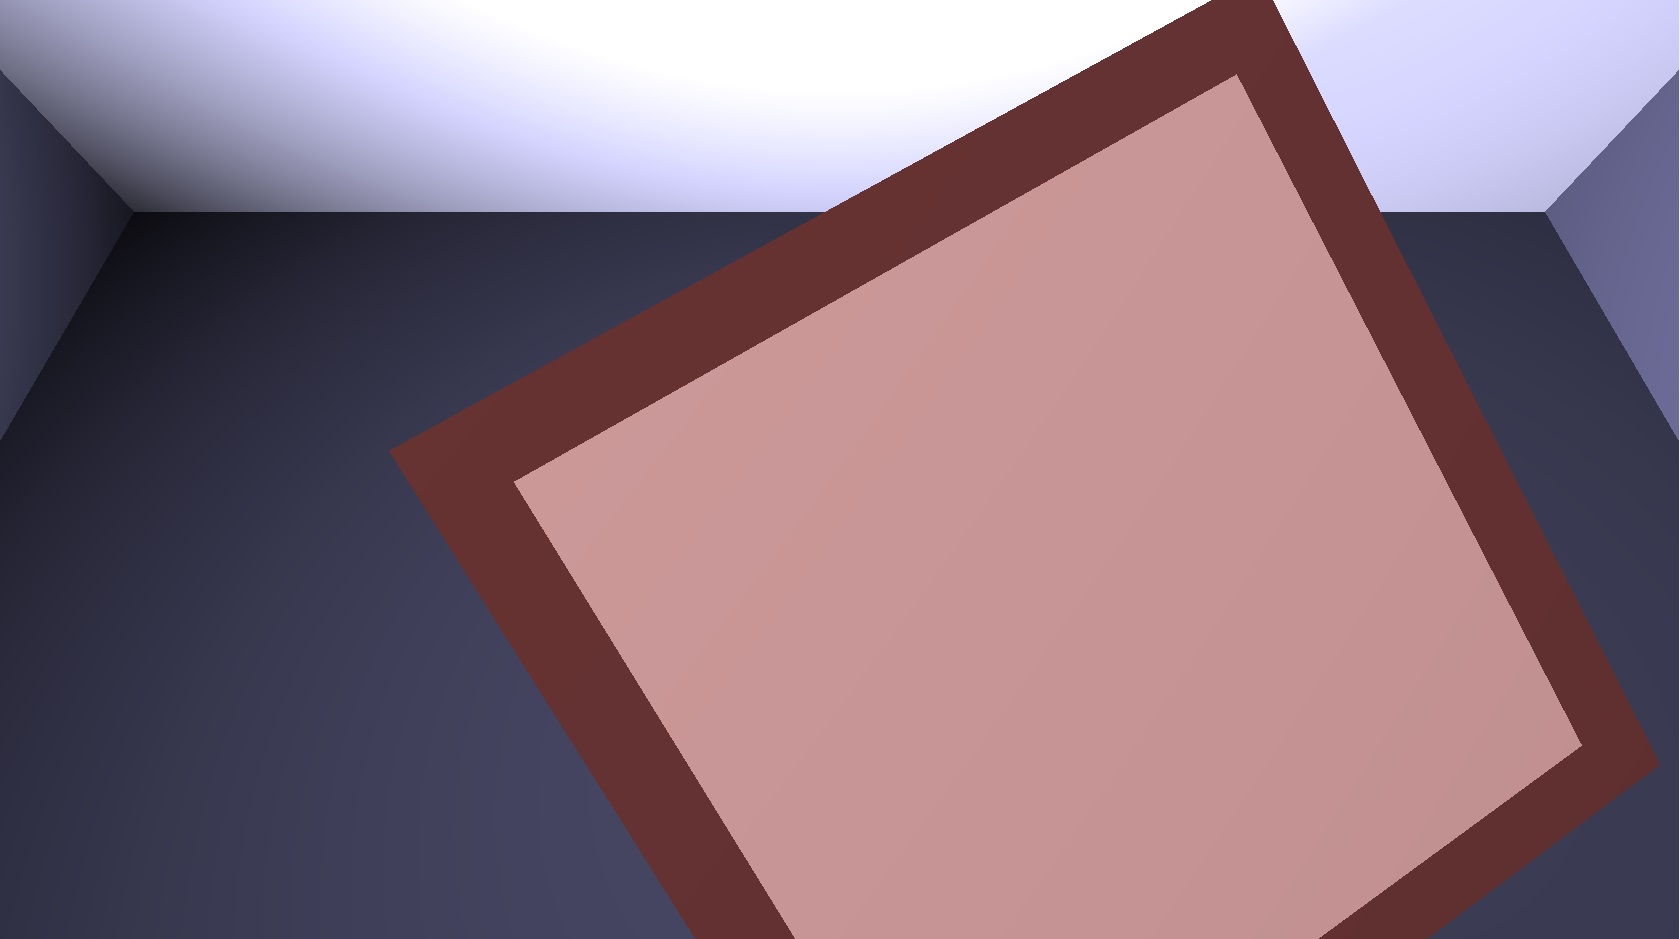
\includegraphics[width=1\linewidth]{test2}
	\caption{Кадр для теста №2}
	\label{fig:test2}
\end{figure}

\begin{figure}
	\centering
	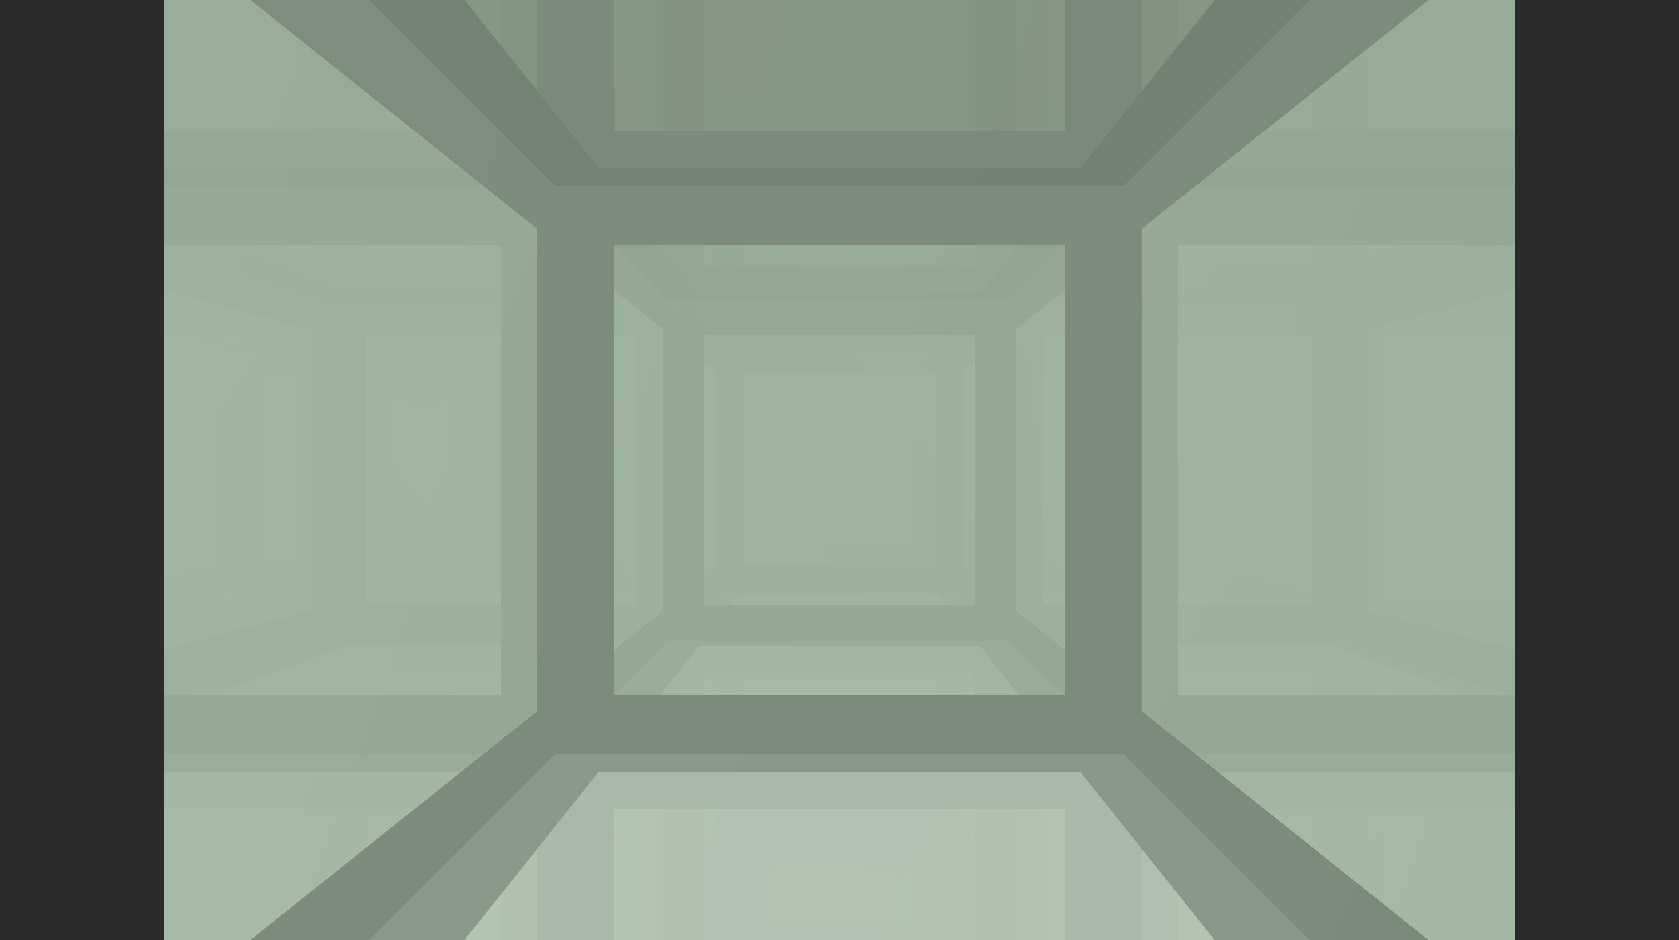
\includegraphics[width=1\linewidth]{test3}
	\caption{Кадр для теста №3}
	\label{fig:test3}
\end{figure}

\begin{figure}
	\centering
	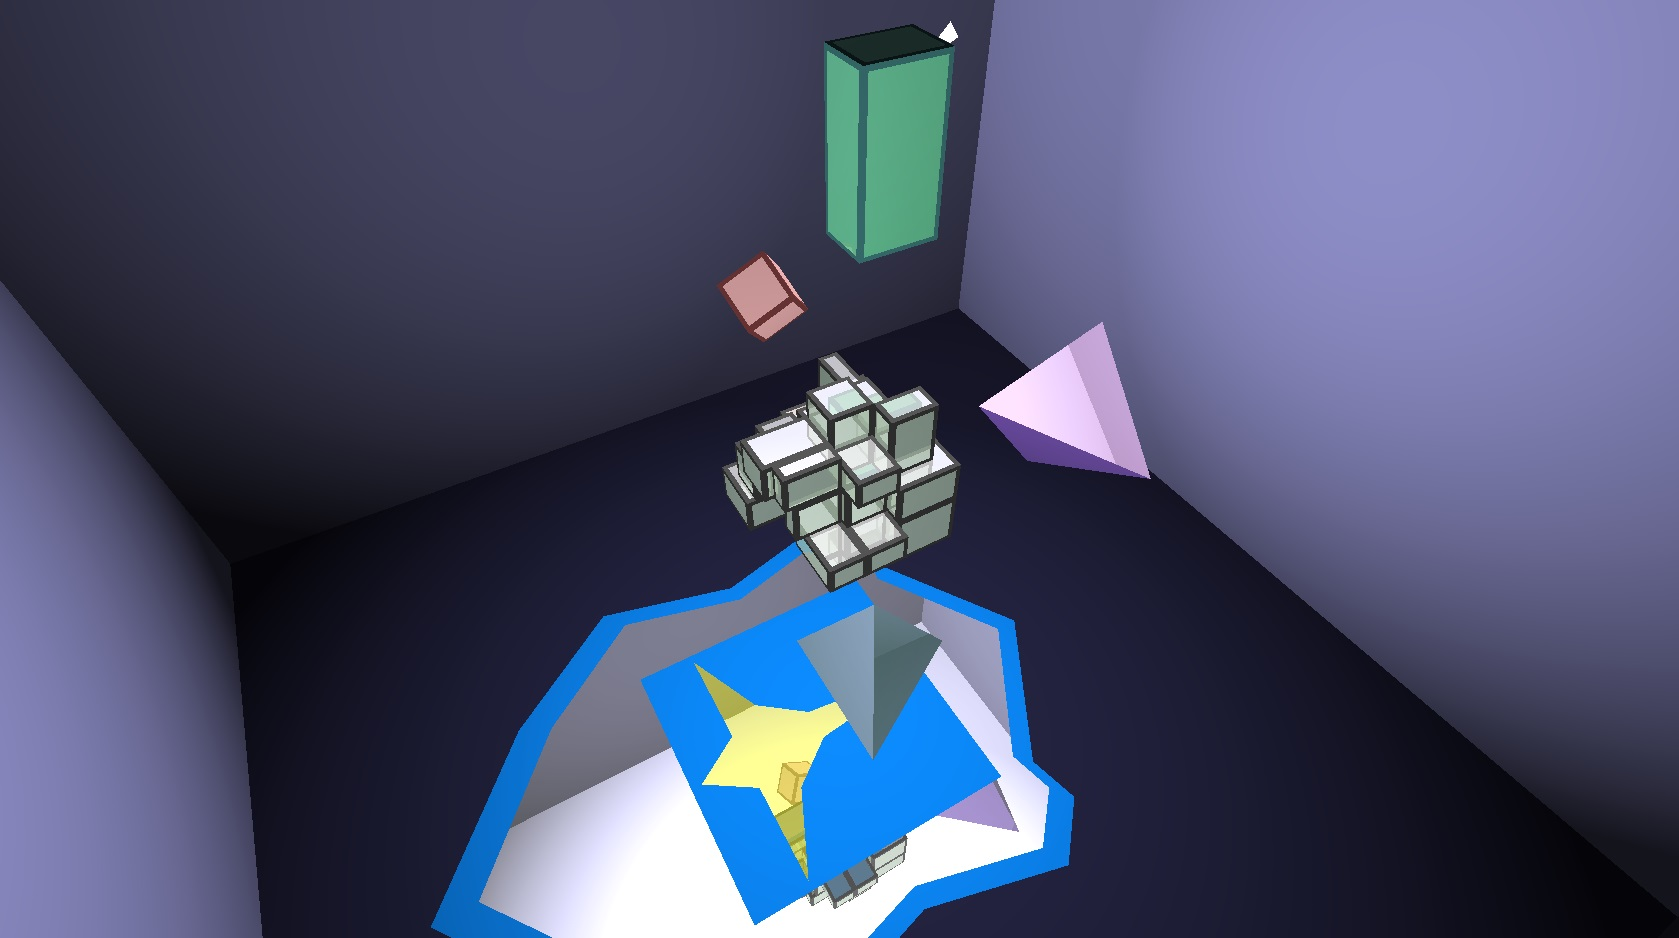
\includegraphics[width=1\linewidth]{test4}
	\caption{Кадр для теста №4}
	\label{fig:test4}
\end{figure}

\begin{figure}
	\centering
	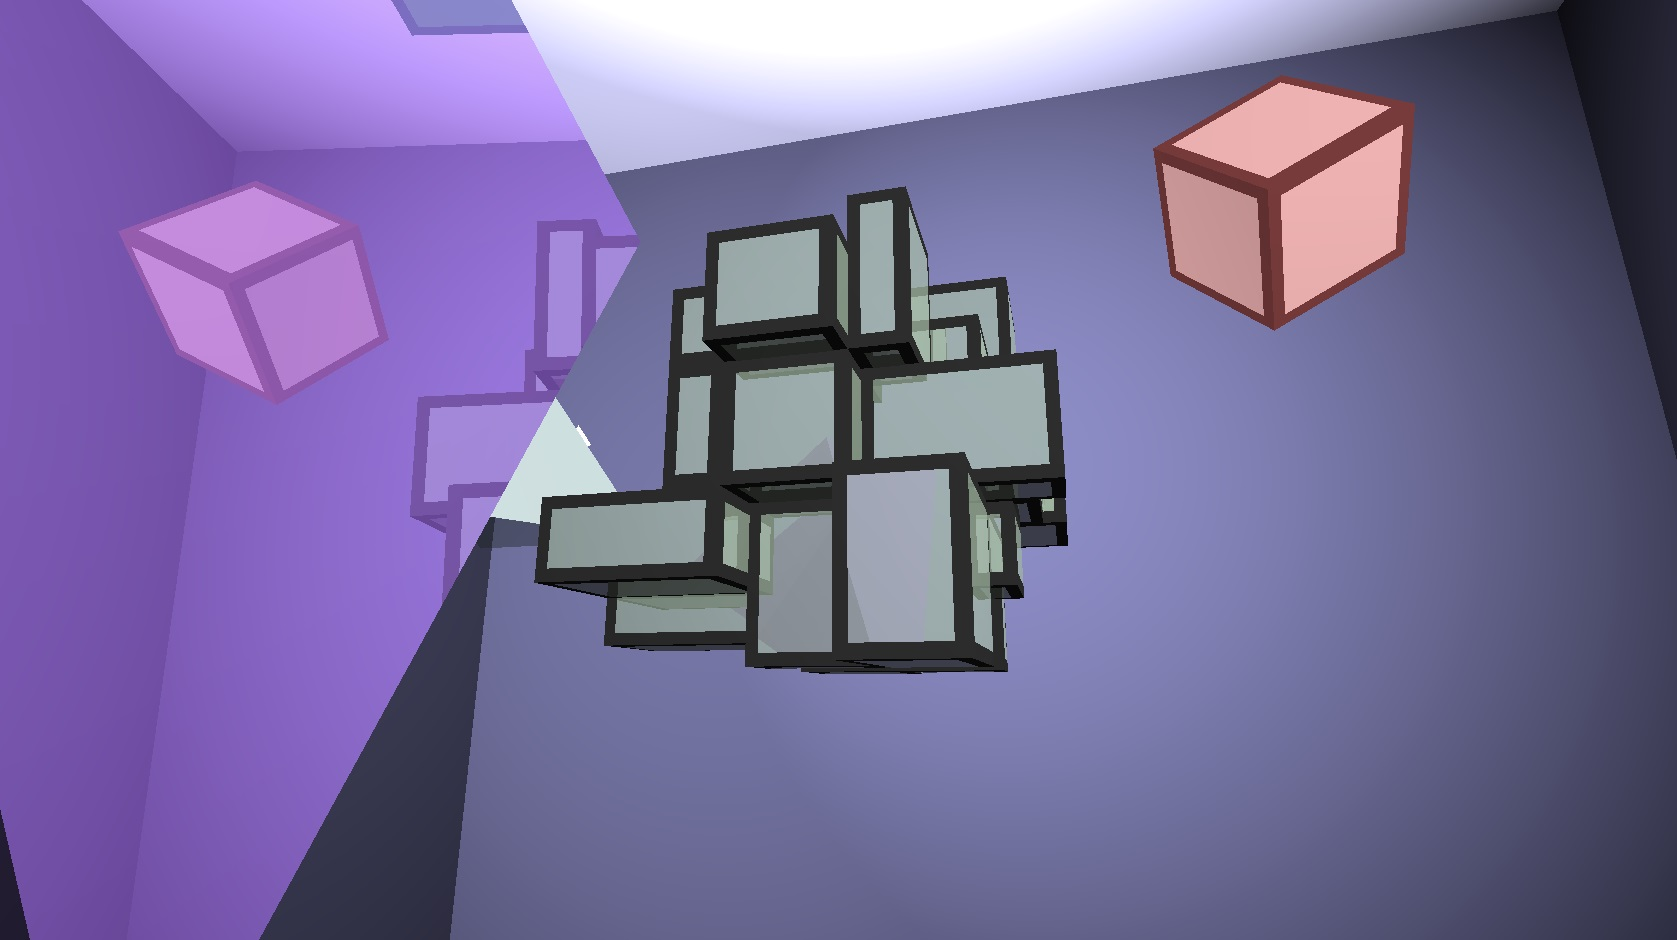
\includegraphics[width=1\linewidth]{test5}
	\caption{Кадр для теста №5}
	\label{fig:test5}
\end{figure}

\begin{figure}
	\centering
	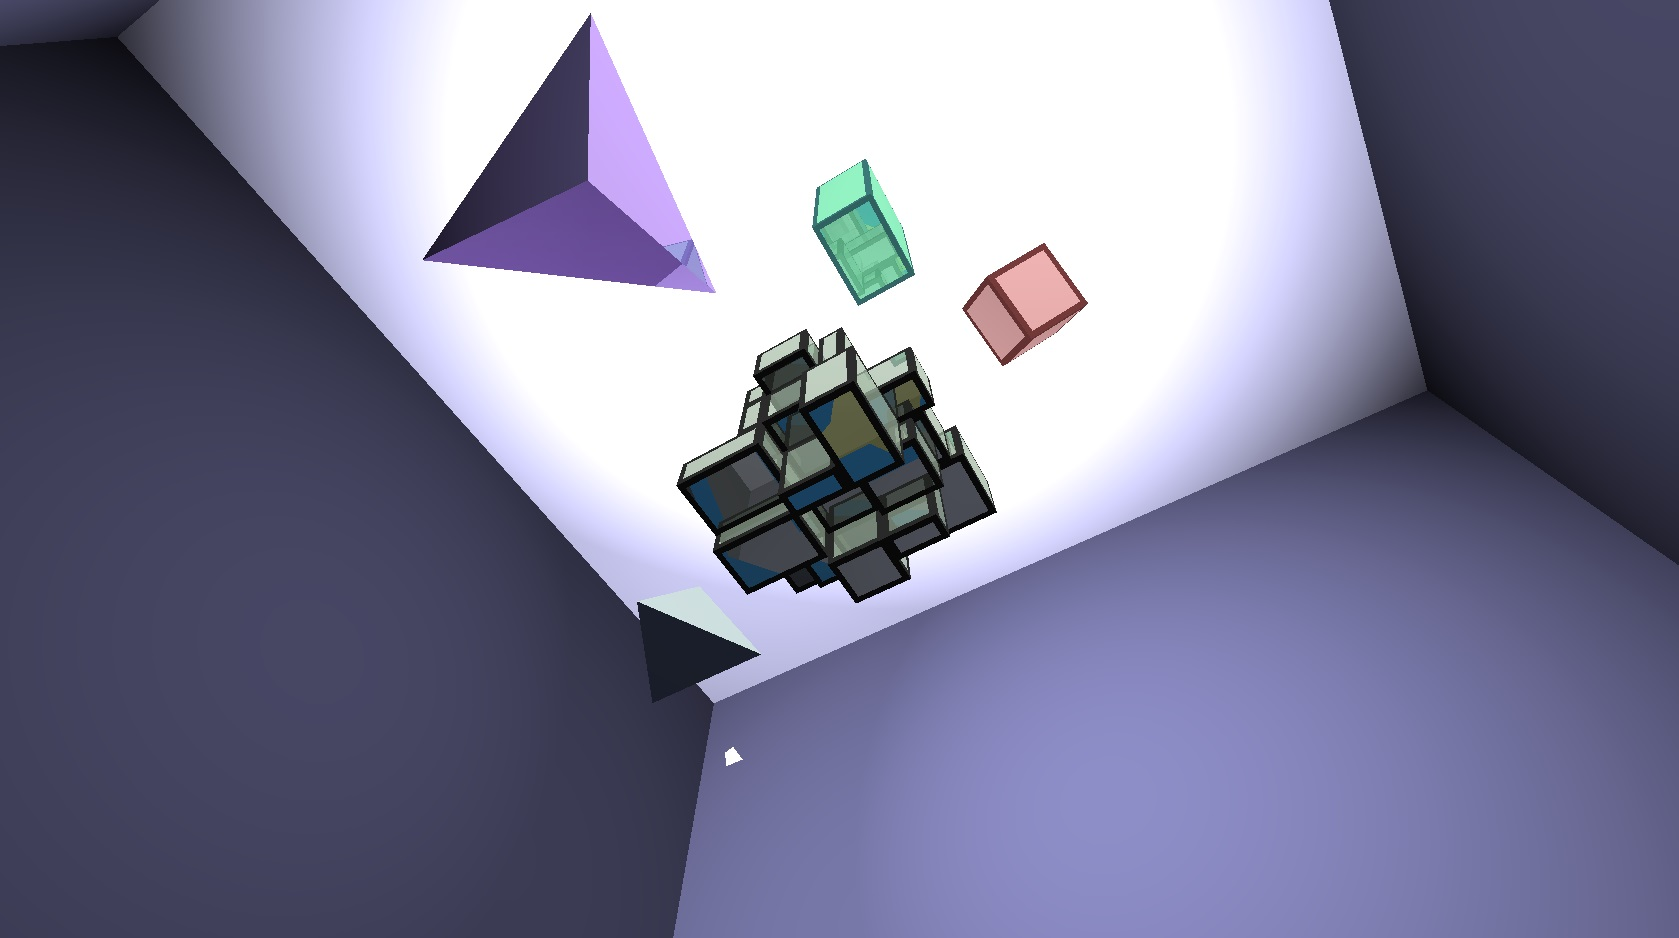
\includegraphics[width=1\linewidth]{test6}
	\caption{Кадр для теста №6}
	\label{fig:test6}
\end{figure}

\subsection{Вывод по разделу}
В исследовательском разделе были проведены замеры времени для шести различных кадров. Из полученных результатов можно сделать вывод о том, что наиболее трудоёмким процессом является рассчёт интенсивности света в точке.
